\section{PS1a: Linear Feedback Shift Register}\label{sec:ps1a}

\subsection{Discussion}\label{sec:ps1a:disc}

Linear Feedback Shift Register is a register that takes a linear function of a previous state as an input. Most commonly, this function is a Boolean exclusive-or (XOR). LFSR performs discrete step operators. Therefore, when we keep shifting the bitstring, we do not get string with 0 at the end. However, for this project we had to XOR 4 bits from the seed and put it at the new spot.
For this project, code step function and generate function.

For step, the function had to shift left once and return the new bit that I XORed. For generate I had to pass an integer value 'k' and run step function k times. Then, update the seed and returns a integer that is step's return value = new value + value * 2.

Also, I had to test the code by using boost unit test framework library.

\begin{figure}[tbh]
	\centering
	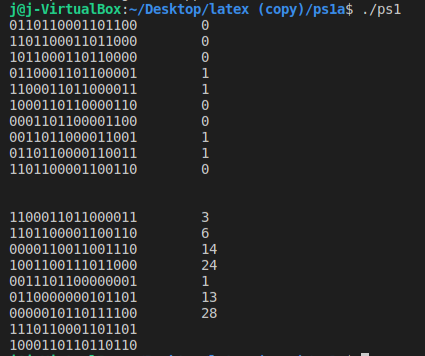
\includegraphics[width=8cm]{ps1a1}
	\caption{The result of main.cpp}
	\label{fig:PS1a Result}
\end{figure}

\begin{figure}[tbh]
	\centering
	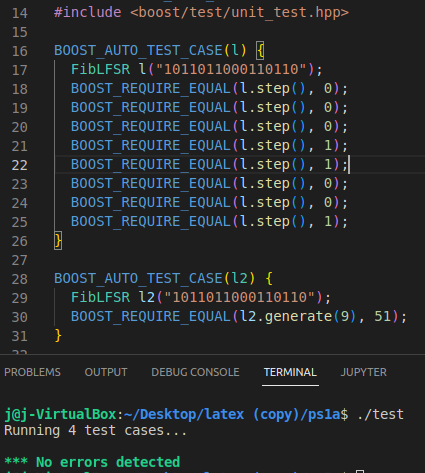
\includegraphics[width=8cm]{ps1a2}
	\caption{The result of test.cpp}
	\label{fig:PS1a Test}
\end{figure}



\subsection{What I accomplished}\label{sec:ps1a:accomplish}

I accomplished to XOR by adding the right index of the string and and gate 0x0001 because I searched on the internet, for XOR, I can power the value or add the values, so I used addition because the logic seemed easier.

\lstinputlisting{ps1a/xorC.cpp}

\subsection{What I already knew}\label{sec:ps1a:knew}

I knew how to use string's .at(index) function to XOR the right index, so it was not hard to shift the bitstring.

\subsection{What I learned}\label{sec:ps1a:learned}

I learned how to code for boost unit test framework library, and it was useful to know because if I have to test it by coding one by one, it will not be as efficient as test framework library.

%\subsection{Challenges}\label{sec:ps0:challenges}

\subsection{Mistakes}\label{sec:ps1a:mistakes}

I got two points off because I had to make two tests by myself, but I did not know that. However, I made it for PSXa and got my points back.

\subsection{Codebase}\label{sec:ps1a:code}
Makefile
\lstinputlisting[language=Make]{ps1a/Makefile}
main.cpp
\lstinputlisting{ps1a/main.cpp}
FibLFSR.cpp
\lstinputlisting{ps1a/FibLFSR.cpp}
FibLFSR.hpp
\lstinputlisting{ps1a/FibLFSR.hpp}
test.cpp
\lstinputlisting{ps1a/test.cpp}

\newpage
